\documentclass[12pt,a4paper]{amsart}
\usepackage[slovene]{babel}
%\usepackage[cp1250]{inputenc}
\usepackage[T1]{fontenc}
\usepackage[utf8]{inputenc}
\usepackage{amsmath,amssymb,amsfonts}
\usepackage{url}
\usepackage[normalem]{ulem}
\usepackage[dvipsnames,usenames]{color}
\usepackage{graphicx}

% Oblika strani
\textwidth 15cm
\textheight 24cm
\oddsidemargin.5cm
\evensidemargin.5cm
\topmargin-5mm
\addtolength{\footskip}{10pt}
\pagestyle{plain}
\overfullrule=15pt % oznaci predlogo vrstico


% Ukazi za matematična okolja
\theoremstyle{definition} % tekst napisan pokončno
\newtheorem{definicija}{Definicija}[section]
\newtheorem{primer}[definicija]{Primer}
\newtheorem{opomba}[definicija]{Opomba}

\renewcommand\endprimer{\hfill$\diamondsuit$}


\theoremstyle{plain} % tekst napisan poševno
\newtheorem{lema}[definicija]{Lema}
\newtheorem{izrek}[definicija]{Izrek}
\newtheorem{trditev}[definicija]{Trditev}
\newtheorem{posledica}[definicija]{Posledica}


% Za številske mnozice uporabi naslednje simbole
\newcommand{\R}{\mathbb R}
\newcommand{\N}{\mathbb N}
\newcommand{\Z}{\mathbb Z}
\newcommand{\C}{\mathbb C}
\newcommand{\Q}{\mathbb Q}

% Ukaz za slovarsko geslo
\newlength{\odstavek}
\setlength{\odstavek}{\parindent}
\newcommand{\geslo}[2]{\noindent\textbf{#1}\hspace*{3mm}\hangindent=\parindent\hangafter=1 #2}


\newcommand{\program}{Finančna matematika} 
\newcommand{\imeavtorja}{Neža Kržan} 
\newcommand{\imementorja}{izr. prof. Jaka Smrekar} 
\newcommand{\naslovdela}{Statistika v kazenskem pravu}
\newcommand{\letnica}{2023} %letnica diplome


\begin{document}

%%%%%%%%%%%%%%%%%%%%%%%%%%%%%%%%%%%%%%%%%%%%%%%%%%%%%%%%%%%%%%%%%%%%%%%%%%%%%%%%%%%%%%%%%%%%%%%%%%%%%%%%%%%%%%%%%%%%%%%%%%%%%%%%%%%%%%%%%%%%
\thispagestyle{empty}
\noindent{\large
UNIVERZA V LJUBLJANI\\[1mm]
FAKULTETA ZA MATEMATIKO IN FIZIKO\\[5mm]
\program\ -- 1.~stopnja}
\vfill

\begin{center}{\large
\imeavtorja\\[2mm]
{\bf \naslovdela}\\[10mm]
Delo diplomskega seminarja\\[1cm]
Mentor: \imementorja}
\end{center}
\vfill

\noindent{\large
Ljubljana, \letnica}
\pagebreak

%%%%%%%%%%%%%%%%%%%%%%%%%%%%%%%%%%%%%%%%%%%%%%%%%%%%%%%%%%%%%%%%%%%%%%%%%%%%%%%%%%%%%%%%%%%%%%%%%%%%%%%%%%%%%%%%%%%%%%%%%%%%%%%%%%%%%%%%%%%%
\thispagestyle{empty}
\tableofcontents
\pagebreak

%%%%%%%%%%%%%%%%%%%%%%%%%%%%%%%%%%%%%%%%%%%%%%%%%%%%%%%%%%%%%%%%%%%%%%%%%%%%%%%%%%%%%%%%%%%%%%%%%%%%%%%%%%%%%%%%%%%%%%%%%%%%%%%%%%%%%%%%%%%%
\thispagestyle{empty}
\begin{center}
{\bf \naslovdela}\\[3mm]
{\sc 
V diplomski nalogi se bom osredotočila na statistiko v kazenskem pravu in na zmote, ki se pojavljajo pri uporabi le te, zaradi pomanjkanja
znanja statistike pri odvetnikih, sodnikih in poroti. Osredotočila se bom na uporabo Bayesove statistike v kazenskih postopkih oziroma na izračune,
ki izhajajo iz Bayesove statistike in jo primerjala z drugimi metodami. V nadaljevanju bom opisala in razložila dve najpogostejši zmoti, prva
je Tožilčeva zmota, ki je dobro znan statistični problem, druga večja, ki pa izhaja iz prve, pa je Zmota obrambnega odvetnika. Ker je uporaba
statistike in verjetnostnega računa čedalje pogostejša v sodnih postopkih, bom na koncu pregledala resničen primer sodbe medicinski sestri Lucii de Berk.
}
\end{center}
% tekst povzetka v slovenscini
%V povzetku na kratko opišite vsebinske rezultate dela. Sem ne sodi razlaga organizacije dela -- v katerem poglavju/razdelku je kaj, pač pa le opis vsebine.
\vfill
\begin{center}
{\bf Angleski naslov dela}\\[3mm] % prevod slovenskega naslova dela 
{\sc Abstract}
\end{center}
% tekst povzetka v anglescini
%Prevod zgornjega povzetka v angleščino.

\vfill\noindent
{\bf Math. Subj. Class. (2010):} navedite vsaj eno klasifikacijsko oznako -- dostopne so na \url{www.ams.org/mathscinet/msc/msc2010.html}  \\[1mm]  
{\bf Ključne besede:} navedite nekaj ključnih pojmov, ki nastopajo v delu  \\[1mm]  
{\bf Keywords:} angleški prevod ključnih besed
\pagebreak

%%%%%%%%%%%%%%%%%%%%%%%%%%%%%%%%%%%%%%%%%%%%%%%%%%%%%%%%%%%%%%%%%%%%%%%%%%%%%%%%%%%%%%%%%%%%%%%%%%%%%%%%%%%%%%%%%%%%%%%%%%%%%%%%%%%%%%%%%%%%
%%%%%%%%%%%%%%%%%%%%%%%%%%%%%%%%%%%%%%%%%%%%%%%%%%%%%%%%%%%%%%%%%%%%%%%%%%%%%%%%%%%%%%%%%%%%%%%%%%%%%%%%%%%%%%%%%%%%%%%%%%%%%%%%%%%%%%%%%%%%
%%%%%%%%%%%%%%%%%%%%%%%%%%%%%%%%%%%%%%%%%%%%%%%%%%%%%%%%%%%%%%%%%%%%%%%%%%%%%%%%%%%%%%%%%%%%%%%%%%%%%%%%%%%%%%%%%%%%%%%%%%%%%%%%%%%%%%%%%%%%%%
%%%%%%%%%%%%%%%%%%%%%%%%%%%%%%%%%%%%%%%%%%%%%%%%%%%%%%%%%%%%%%%%%%%%%%%%%%%%%%%%%%%%%%%%%%%%%%%%%%%%%%%%%%%%%%%%%%%%%%%%%%%%%%%%%%%%%%%%%%%%%%
\section{Koncept verjetnosti}
\begin{definicija}
    Naj bo $H$ nek dogodek in $\bar{H}$ negacija oziroma komplement dogodka $H$. Dogodka $H$ in $\bar{H}$ sta znana kot komplementarna dogodka.
\end{definicija}
Pogosto se opravlja primerjava verjetnosti dokazov na podlagi dveh konkurenčnih predlogov, in sicer predloga tožilca in predloga obrambe.\\
$H_p \dots$ trditev, ki jo predlaga tožilstvo;\\
$H_d \dots$ trditev, ki jo predlaga obramba;\\
Hipoteze se lahko dopolnjujejo na enak način kot dogodki - ena in samo ena je lahko resnična, med seboj se izključujejo. Ni nujno, da so izbrane tako,
da zajemajo vse možne razlage dokazov. Dve hipotezi lahko označujeta komplementarne dogodke(npr. resnično kriv in resnično nedolžen), vendar pa se lahko zgodi,
da se označena dogodka ne dopolnjujeta. \\\\
Koncept verjetnosti je pomemben pri ocenjevanju dokazov, saj se le ti ocenjujejo glede na njihov vpliv na verjetnost določene domneve o interesni
osebi(v nadaljevanju PoI) (preden pride do sojenja) ali obdolžencu(medtem, ko sojenje poteka). Zanima nas vpliv dokazov na verjetnost krivde($H_p$) in
nedolžnosti($H_d$) osumljenca. Gre za dopolnjujoča se dogodka in razmerje verjetnosti teh dveh dogodkov,
\begin{equation}
   \frac{P(H_p)}{P(H_d)}, \vspace{2mm}
\end{equation}
je verjetnost proti nedolžnosti ali verjetnost za krivdo. Ob upoštevanju dodatnih informacij $E$(oz. dokazov), je razmerje
\begin{equation}
   \frac{P(H_p \lvert E)}{P(H_d \lvert E)} \vspace{2mm},
\end{equation}
verjetnost v prid krivdi ob upoštevanju informacij $E$.\\\\
Občasno se zgodi, da predloga tožilstva in obrambe nista komplementarna in v takih primerih ni mogoče določiti $P(H_p)$ ali $P(H_d)$, ampak samo
vpliv statistike, znane kot razmerje verjetnosti(angl. Likelihood Ratio; oznaka LR).

%%%%%%%%%%%%%%%%%%%%%%%%%%%%%%%%%%%%%%%%%%%%%%%%%%%%%%%%%%%%%%%%%%%%%%%%%%%%%%%%%%%%%%%%%%%%%%%%%%%%%%%%%%%%%%%%%%%%%%%%%%%%%%%%%%%%%%%%%%%%%%
%%%%%%%%%%%%%%%%%%%%%%%%%%%%%%%%%%%%%%%%%%%%%%%%%%%%%%%%%%%%%%%%%%%%%%%%%%%%%%%%%%%%%%%%%%%%%%%%%%%%%%%%%%%%%%%%%%%%%%%%%%%%%%%%%%%%%%%%%%%%%%
\section{Razmerje verjetnosti(angl. Likelihood Ratio)}

%%%%%%%%%%%%%%%%%%%%%%%%%%%%%%%%%%%%%%%%%%%%%%%%%%%%%%%%%%%%%%%%%%%%%%%%%%%%%%%%%%%%%%%%%%%%%%%%%%%%%%%%%%%%%%%%%%%%%%%%%%%%%%%%%%%%%%%%%%%%%%
\subsection{Opredelitev}
V Bayesovi formuli %napiš si številko%
nadomestimo $H$ z $\bar{H}$ in enakovredna različica Bayesovega izreka je
\begin{equation}
   P(\bar{H} \lvert E) = \frac{P(E \lvert \bar{H})P(\bar{H})}{P(E)}, \vspace{2mm}
\end{equation}
kjer $P(E) \ne 0$.\\\\
Če prvo enačbo delimo z drugo dobimo verjetnostno obliko Bayesovega izreka
\begin{equation}
   \frac{P(H \lvert E)}{P(\bar{H} \lvert E)} = \frac{P(E \lvert H)}{P(E \lvert \bar{H})} \times \frac{P(H)}{P(\bar{H})}. \vspace{2mm}
\end{equation}
Leva stran je verjetnost dogodka $H$ ob pogoju, da se je zgodil dogodek $E$. Pogojna verjetnost na desni strani dogodka, $H$ in $\bar{H}$,
sta v števcu in imenovalcu različna, medtem ko je dogodek $E$, katerega verjetnost nas zanima, enak. Na koncu pa imamo verjetnost v
korist dogodka $H$ brez kakršnihkoli informacij o $E$.\\
\begin{definicija}
   Razmerje
   \begin{equation}
       \frac{P(E \lvert H)}{P(E \lvert \bar{H})} \vspace{2mm}
   \end{equation}
   se imenuje razmerje verjetnosti(angl. Likelihood Ratio). \\
\end{definicija}
Oglejmo si dogodka $E$ in $H$, ter njuni dopolnitvi. Razmerje verjetnosti je tu razmerje verjetnosti $E$, ko je $H$ resničen in verjetnosti $E$,
ko je $H$ neresničen. Da bi upoštevali učinek $E$ na verjetnost $H$, tj. da bi
\[
   \frac{P(H)}{P(\bar{H})} \vspace{2mm}
\]
spremenili v
\[
   \frac{P(H \lvert E)}{P(\bar{H} \lvert E)}, \vspace{2mm}
\]
prvo pomnožimo z razmerjem verjetnosti. Verjetnost
\[
   \frac{P(H)}{P(\bar{H})} \vspace{2mm}
\]
je znana kot predhodna verjetnost v korist H, verjetnost
\[
   \frac{P(H \lvert E)}{P(\bar{H} \lvert E)} \vspace{2mm}
\]
pa je znana kot posteriorna verjetnost v korist $H$. Razlika med $P(E \lvert H)$ in $P(H \lvert E)$ je bistvena.Pri proučevanju vpliva
$E$ na $H$ je treba upoštevati tako verjetnost $E$, ko je $H$ resničen in ko je $H$ neresničen. Pogosta napaka(zmota prenesene pogojne
verjetnosti) je, da dogodek $E$, ki je malo verjeten, če je $\bar{H}$ resničen, pomeni dokaz v prid $H$. Da bi bilo tako, je treba dodatno
zagotoviti, da E ni tako malo verjeten, če je H resničen. Razmerje verjetnosti je potem večje od 1 in pozitivna verjetnost je večja od
predhodne verjetnosti. Torej iz Bayesovega izreka neposredno izhaja, da če je razmerje verjetnosti večje od 1, potem dokaz povečuje
verjetnost krivde (pri čemer višje vrednosti pomenijo večjo verjetnost krivde), če pa je manjše od 1, zmanjšuje verjetnost krivde
(in bolj ko se približuje ničli, manjša je verjetnost krivde).\\

%%%%%%%%%%%%%%%%%%%%%%%%%%%%%%%%%%%%%%%%%%%%%%%%%%%%%%%%%%%%%%%%%%%%%%%%%%%%%%%%%%%%%%%%%%%%%%%%%%%%%%%%%%%%%%%%%%%%%%%%%%%%%%%%%%%%%%%%%%%%%%
\subsection{Razmerje verjetnosti v kazenskem pravu}
Obravnavajmo obliko Bayesovega izreka o verjetnosti v forenzičnem kontekstu ocenjevanja vrednosti nekaterih dokazov. Naj bo:\\
$H_p \dots$ interesna oseba(PoI) oz. obtoženec je resnično kriv - nadomestimo $H$;\\
$H_d \dots$ interesna oseba(PoI) je resnično nedolžen - nadomestimo $\bar{H}$;\\
$Ev \dots$ obravnavani dokaz - nadomestimo dogodek $E$;\\\\
Oblika Bayesovega izreka nato omogoča, da se predhodne verjetnosti(tj, pred predstavitvijo $Ev$) v korist krivde posodobijo v posteriorne
verjetnosti ob upoštevanju $Ev$, na naslednji način:
\[
   \frac{P(H_p \lvert Ev)}{P(H_d \lvert Ev)} = \frac{P(Ev \lvert H_p)}{P(Ev \lvert H_d)} \times \frac{P(H_p)}{P(H_d)}. \vspace{2mm}
\]
Ob upoštevanju informacij o ozadju $I$, dobimo zapis
\[
   \frac{P(H_p \lvert Ev, I)}{P(H_d \lvert Ev, I)} = \frac{P(Ev \lvert H_p, I)}{P(Ev \lvert H_d, I)} \times \frac{P(H_p \lvert I)}{P(H_d \lvert I)}. \vspace{2mm}
\]
Pri vrednotenju dokazov $Ev$ sta potrebni dve verjetnosti - verjetnost dokazov, če je PoI kriv in glede na informacije o ozadju, ter
verjetnost dokazov, če je PoI nedolžen in glede na informacije o ozadju. Informacije o ozadju so včasih znane kot okvir okoliščin
ali pogojne informacije. \\\\
Da lahko ocenimo oziroma določimo vrednost dokaza potrebujemo razmerje verjetnosti(angl. Likelihood ratio).
\begin{definicija}
   Naj bosta  $H_p$ in $H_d$ dve konkurenčni hipotezi ter $I$ informacije o ozadju. Vrednost $V$ dokaza $Ev$ je podana z
   \[
       V = \frac{P(Ev \lvert H_p, I)}{P(Ev \lvert H_d, I)}, \vspace{2mm}
   \]
   razmerje verjetnosti, ki pretvori predhodne verjetnosti
   \[
       \frac{P(H_p \lvert I)}{P(H_d \lvert I)} \vspace{2mm}
   \]
   v posteriorne verjetnosti
   \[
       \frac{P(H_p \lvert Ev, I)}{P(H_d \lvert Ev, I)}. \vspace{2mm}
   \]
\end{definicija}


\begin{table}[h!]
   \centering
   \caption{Kvalitativna lestvica za poročanje o vrednosti $V$ podpore dokazov za $H_p$ proti $H_d$(Vir: ENFSI, 2015).}
   \label{table:1}
    \begin{tabular}{c c c c}
       \hline
       1 & $< V \le$  & 2 & brez podpore \\
       2 & $< V \le$ & 10 & šibka podpora prvi hipotezi \\
       10 & $< V \le$ & 100 & zmerna podpora prvi hipotezi \\
       100 & $< V \le$ & 1000 & srednje močna podpora prvi hipotezi \\
       1000 & $< V \le$ & 10000 & močna podpora prvi hipotezi \\
       10000 & $< V \le$ & 1000000 & zelo močna podpora prvi hipotezi \\
       1000000 & $< V $ & & izjemno močna podpora prvi hipotezi \\ [1ex]
       \hline
    \end{tabular}
\end{table}


%%%%%%%%%%%%%%%%%%%%%%%%%%%%%%%%%%%%%%%%%%%%%%%%%%%%%%%%%%%%%%%%%%%%%%%%%%%%%%%%%%%%%%%%%%%%%%%%%%%%%%%%%%%%%%%%%%%%%%%%%%%%%%%%%%%%%%%%%%%%%%
\subsection{Utemeljitev uporabe razmerja verjetnosti}
Verjetnostna oblika Bayesovega izreka predstavlja prepričljiv intuitivni argument za uporabo razmerja verjetnosti kot merila vrednosti dokazov.
Obstaja tudi matematični argument, ki opravičuje njegovo uporabo.\\\\
Želimo izmeriti vrednost $V$ dokazov $E$ v prid krivdi $H_p$. Pri tem bo obstajala odvisnost od osnovnih informacij $I$, vendar ta ne bo izrecno
navedena. Predpostavlja se, da je ta vrednost $V$ odvisna samo od verjetnosti $E$ ob pogoju, da je PoI kriv($H_p$), in od verjetnosti $E$ ob pogoju,
da je PoI nedolžen($H_d$). Naj bo $x=P(E \lvert H_p)$ in $y=P(E \lvert H_d)$. Zgornja predpostavka pravi, da je $V = f (x, y)$ za neko funkcijo $f$.
Vzemimo še en dokaz $T$, ki je neodvisen od $E$ in $H_p$ (in s tem $H_d$) in je tak, da je $P(T) = \theta$. Nato
\begin{align}
   P(E,T \lvert H_p) & = \\
   & = P(E \lvert H_p)P(T \lvert H_p) \\
   & = P(E \lvert H_p)P(T)\\
   & = \theta x, \vspace{2mm}
\end{align}
pri čemer iz (6) v (7) upoštevamo neodvisnost dokaza $E$ in $T$ ter iz (7) v (8) vrstico neodvisnost dokaza $T$ in $H_p$. podobno
\[
   P(E,T \lvert H_d)  = \theta y. \vspace{2mm}
\]
Vrednost kombiniranih dokazov $(E, T)$ je enaka vrednosti $E$, saj je bil $T$ predpostavljen kot nepomemben. Vrednost $(E, T)$ je $f(\theta x, \theta y)$,
vrednost $E = V = f (x, y)$. Tako je $f(\theta x, \theta y) = f(x,y)$ za vsako $\theta$ v intervalu $[0,1]$ možnih vrednosti $P(T)$. Razmerje med
$x$ in $y$ v funkciji $f$ ima lahko eno od štirih oblik, odvisno od štirih matematičnih operatorjev +, ×, - in /. Če pogledamo $\frac{x}{y}$ sledi
\[
   f(x,y) = f \big(\frac{x}{y}\big)
   f(\theta x, \theta y) = f(\frac{\theta x}{\theta y}) = f(\frac{x}{y}). \vspace{2mm}
\]
To je enako $f(x,y)$ za vsako $\theta$ v intervalu $[0,1]$. Iz tega sledi, da je $f$ funkcija $\frac{x}{y}$ in torej, da je $V$ funkcija
\[
   \frac{P(E \lvert H_p)}{P(E \lvert H_d)}, \vspace{2mm}
\]
kar je razmerje verjetnosti.\\\\
Verjetnost hipoteze H na podlagi nekega dokaza E je verjetnost, da najdemo E, če je H resnična. Za alternativno hipotezo je LR razmerje obeh
verjetnosti. LR nam pove, katera hipoteza je bolje podprta z dokazi. Kadar sta hipotezi medsebojno izključujoči in izčrpni, nam LR pove več.
V tem primeru, če je verjetnost H večja od verjetnosti alternative, lahko sklepamo tudi, da se verjetnost H zaradi najdbe E poveča, medtem ko se
verjetnost alternative zmanjša. Če je le mogoče, je treba upoštevati verjetnosti za vse razumne alternativne hipoteze (tako da je nabor hipotez
izčrpen). Če se obravnavajo samo nekatere hipoteze, je treba pojasniti, da so predstavljene samo LR za pare teh hipotez. V primerih, ko je treba
združiti več hipotez in/ali več dokazov, se lahko LR bolje uporablja v povezavi z drugimi metodami.\\
Kadar je treba količinsko ovrednotiti skupni učinek več dokazov, ki vključujejo različne povezane hipoteze (kot so hipoteze o ravni vira, ravni
dejavnosti in ravni kaznivega dejanja), poenostavljene rešitve, ki neupravičeno predpostavljajo neodvisnost, niso ustrezne. Grafični prikazi dokazov
so lahko v veliko pomoč pri modeliranju odvisnosti. Obstaja interaktivna programska oprema za izvajanje izračunov na grafičnih modelih(Bayesovih mrežah),
ki uporabnikom omogoča, da raziščejo vplive različnih predpostavk. Čeprav je takšne metode težko uvesti neposredno na sodišču, so koristne za sintezo
dokazov v katerikoli fazi preiskave pred sojenjem.\\\\
Ocena vrednosti razmerja verjetnosti je lahko podvržena številnim virom negotovosti, vključno s kakovostjo podatkov, pridobljenih z analizami, ki jih
opravijo forenzični znanstveniki, izbiro kontrolnega vzorca in najdenih predmetov, ki jih lahko vzamejo različni preiskovalci ali analizirajo različni
analitiki ali laboratoriji. Ocena znanstvenih dokazov na sodišču pogosto zahteva kombinacijo podatkov o pojavu ciljnih značilnosti skupaj z osebnim poznavanjem
okoliščin iz določenega primera. Jasno je, da ima vsaka ocena verjetnosti, ki se nanaša na določen primer, tudi če jo obravnavamo v obliki frekvence, sestavino,
ki temelji na osebnem znanju. Drugi viri negotovosti vključujejo pridobivanje predhodnih verjetnosti, pogojenih z razpoložljivim znanjem, ali celo
izvajanje numeričnih postopkov za razreševanje računskih težav. Poročilo o vrednosti razmerja verjetnosti vključuje merilo njegove natančnosti, na primer z
navedbo številčnega razpona vrednosti za verjetnost dokazov na podlagi konkurenčnih predlogov in s tem številčnega razpona vrednosti za razmerje verjetnosti.
Vendar sta vrednost dokaza in moč posameznikovega prepričanja o vrednosti različna pojma in se ne smeta združevati v intervalu ali povzročiti spremembe
vrednosti dokaza, kot se to na primer zgodi z navedbo spodnje meje neke poljubno izbrane ravni. V praksi je za kriminalistično preiskavo na voljo en niz
podatkov o ozadju, ki so značilni za člane določene relevantne populacije, en niz kontrolnih podatkov in en niz izterjanih podatkov. Zato je za vrednotenje
dokazov z določenim statističnim modelom na voljo ena sama vrednost $V$ za povezano razmerje verjetnosti. Ponovno je treba upati, da so vsi različni kontrolni
vzorci in pridobljeni podatki dovolj reprezentativni za populacije, iz katerih so bili izbrani, tako da se bodo razmerja verjetnosti po vrednosti le malo
razlikovala.

%%%%%%%%%%%%%%%%%%%%%%%%%%%%%%%%%%%%%%%%%%%%%%%%%%%%%%%%%%%%%%%%%%%%%%%%%%%%%%%%%%%%%%%%%%%%%%%%%%%%%%%%%%%%%%%%%%%%%%%%%%%%%%%%%%%%%%%%%%%%%%
\subsection{Bayesov faktor(angl. Bayes' Factor) in razmerje verjetnosti}
V forenziki se ta dva pojma, kljub pogostejši uporabi Bayesovega faktorja(BF), pogosto obravnavata kot sinonima. Bayesov faktor je glavni
element Bayesove metodologije za primerjavo konkurenčnih predlogov. Opredeljen je kot sprememba, ki jo povzročijo novi dokazi (podatki) v
verjetnosti pri prehodu od predhodne k posteriorni porazdelitvi v korist enega predloga k drugemu. Da se pokazati, da je razmerje verjetnosti
poseben primer Bayesovega faktorja, kadar so konkurenčne hipoteze parametrizirane z enim samim parametrom (tj. preprosta hipoteza). Vendar pa
lahko pride do primerov, ko se primerjajo sestavljene hipoteze. V takem primeru je Bayesov faktor razmerje dveh mejnih verjetnosti pri konkurenčnih
hipotezah in se zdi, da ni več odvisen samo od podatkov.
%Če je razmerje verjetnosti enako ali blizu 1, potem E nima nobene prave vrednosti, saj ne povečuje niti ne zmanjšuje verjetnosti krivde.(bayesovo razmerje verjetnosti)

%%%%%%%%%%%%%%%%%%%%%%%%%%%%%%%%%%%%%%%%%%%%%%%%%%%%%%%%%%%%%%%%%%%%%%%%%%%%%%%%%%%%%%%%%%%%%%%%%%%%%%%%%%%%%%%%%%%%%%%%%%%%%%%%%%%%%%%%%%%%%%
%%%%%%%%%%%%%%%%%%%%%%%%%%%%%%%%%%%%%%%%%%%%%%%%%%%%%%%%%%%%%%%%%%%%%%%%%%%%%%%%%%%%%%%%%%%%%%%%%%%%%%%%%%%%%%%%%%%%%%%%%%%%%%%%%%%%%%%%%%%%%%
\section{Bayesova statistika}
Bayesova statistika je statistična veja, ki nam s pomočjo matematičnih pristopov omogoča uporabo verjetnosti pri reševanju statističnih
problemov. V svoje modele vključuje pogojno verjetnost, katero izračunamo z uporabo Bayesovega pravila. \\\\
Zlasti Bayesovo sklepanje razlaga verjetnost kot merilo verjetnosti ali zaupanja, ki ga lahko ima posameznik glede nastanka določenega dogodka.
O nekem dogodku lahko že imamo predhodno prepričanje oziroma apriorno prepričanje, ki pa se lahko spremeni, ko se pojavijo novi dokazi. Bayesova
statistika nam daje matematične modele za vključevanje naših apriornih prepričanj in dokazov za ustvarjanje novih prepričanj oziroma za
pridobitev aposteriornega prepričanja, ki se lahko uporabi za kasnejše odločitve.\\\\
Bayesova analiza je standardna metoda za posodabljanje verjetnosti po opazovanju več dokazov, zato je zelo primerna za sintezo dokazov.
Vsakdo, ki mora presoditi o hipotezi, kot je "krivda" (vključno s preiskovalci pred sojenjem, sodniki, porotami), neformalno začne z nekim
predhodnim prepričanjem o hipotezi in ga posodablja, ko se dokazi ponovno pojavijo. Včasih lahko obstajajo celo objektivni podatki, na katerih temelji
predhodna verjetnost. Pri uporabi Bayesovega sklepanja morajo statistiki utemeljiti predhodne predpostavke, kadar je to mogoče, na primer z
uporabo zunanjih podatkov; v nasprotnem primeru morajo uporabiti razpon vrednosti predpostavk in analizo občutljivosti, da preverijo zanesljivost rezultata
glede na te vrednosti.

%%%%%%%%%%%%%%%%%%%%%%%%%%%%%%%%%%%%%%%%%%%%%%%%%%%%%%%%%%%%%%%%%%%%%%%%%%%%%%%%%%%%%%%%%%%%%%%%%%%%%%%%%%%%%%%%%%%%%%%%%%%%%%%%%%%%%%%%%%%%%%
\subsection{Beyesovo pravilo}
Bayesovo sklepanje temelji na Bayesovem pravilu, ki izraža verjetnost nekega dogodka z verjetnostjo dveh dogodkov in obrnejnje pogojne
verjetnosti. Pogojna verjetnost predstavlja verjetnost dogodka, glede na drug dogodek.
\begin{definicija}
   Pogojna verjetnost dogodka H, glede na dogodek E, je
   \begin{equation}\label{eq:pogojna}
   P(H \lvert E) = \frac{P(H \cap E)}{P(E)}, \vspace{2mm}
   \end{equation}
   ob predpostavki, da je $P(E) > 0$.
\end{definicija}
Formula \eqref{eq:pogojna} pove, da je verjetnost dogodka H ob pogoju, da se je zgodil dogodek E, enaka razmerju verjetnosti, da se
zgodita oba dogodka in verjetnosti, da se je zgodil dogodek E.
Potem pogojno verjetnost uporabimo še v števcu formule \eqref{eq:pogojna} in dobimo Bayesovo pravilo:
\begin{equation}\label{eq:bpravilo}
   P(H \lvert E) = \frac{P(E \lvert H) \times P(H)}{P(E)}, \vspace{2mm}
\end{equation}  
verjetnost dogodka E lahko še razpišemo in dobimo:
\begin{equation}\label{eq:b_pravilo}
   P(H \lvert E) = \frac{P(E \lvert H) \times P(H)}{P(E \lvert H)P(H) + P(E \lvert \neg H)P(\neg H)}. \vspace{2mm}
\end{equation} \\\\
Obstaja še ena formulacija Bayesovega pravila, ki olajša izračune in je pogosto uporabljena pri Bayesovi analizi DNK dokazov:
\begin{equation}\label{eq:b_pravilo_DNK}
   \frac{P(H \lvert E)}{P(\neg H \lvert E)} = \frac{P(E \lvert H)}{P(E \lvert \neg H)} \times \frac{P(H)}{P(\neg H)}. \vspace{2mm}
\end{equation}

%%%%%%%%%%%%%%%%%%%%%%%%%%%%%%%%%%%%%%%%%%%%%%%%%%%%%%%%%%%%%%%%%%%%%%%%%%%%%%%%%%%%%%%%%%%%%%%%%%%%%%%%%%%%%%%%%%%%%%%%%%%%%%%%%%%%%%%%%%%%%%
\subsection{Beyesovo posodabljanje}
Bayesovo pravilo se razlikuje od Bayesovega posodabljanja. Prvo je matematični izrek, drugo pa logična trditev, kako se sčasoma posodabljajo
apriorne verjetnosti dokazov glede na novo zbrane dokaze oziroma prepričanja.\\\\
Bayesovo posodabljanje pravi:
\begin{trditev}
Če se dogodek E zgodi ob času $t_1 > t_0$, potem je $P_1(H) = P_0(H \lvert E)$.
\end{trditev}
Ob času $t_0$ dogodku H dodelimo verjetnost $P_0(H)$; to se imenuje predhodna verjetnost oziroma apriorna verjetnost. Ko se zgodi dogodek E
ob času $t_1$, ki vpliva na naša prepričanja o dogodku H, Bayesovo posodabljanje pravi, da je potrebno apriorno verjetnost dogodka H v času $t_1$
enačiti z pogojno verjetnostjo dogodka H glede na dogodek E v času $t_0$. \\\\
Recimo, da je dogodek H neka hipoteza oziroma prepričanje o zločinu in dogodek E dokazi, zbrani za ta zložin. Pri Bayesovem posodabljanju je videti,
kot da je dokaz E nesporno resničen. Z drugimi besedami, predpostavka je, da moramo imeti po zbiranju dokazov E stopnjo zaupanja v E enako 1,
torej če so dokazi zbarni v času $t_1$, je $P_1(E)=1$.

%%%%%%%%%%%%%%%%%%%%%%%%%%%%%%%%%%%%%%%%%%%%%%%%%%%%%%%%%%%%%%%%%%%%%%%%%%%%%%%%%%%%%%%%%%%%%%%%%%%%%%%%%%%%%%%%%%%%%%%%%%%%%%%%%%%%%%%%%%%%%%
%%%%%%%%%%%%%%%%%%%%%%%%%%%%%%%%%%%%%%%%%%%%%%%%%%%%%%%%%%%%%%%%%%%%%%%%%%%%%%%%%%%%%%%%%%%%%%%%%%%%%%%%%%%%%%%%%%%%%%%%%%%%%%%%%%%%%%%%%%%%%%
\section{Beyesova analiza}
V kazenskih zadevah želimo vedeti, ali je obtoženec kriv ali ne. Če imamo torej na voljo dokaz $E$, nas zanima pogojna verjetnost
\[
   P(kriv \lvert E), \vspace{2mm}
\]
pri čemer nam je lahko v pomoč Bayesovo pravilo. To v teoriji drži, čeprav je v praksi izračun verjetnostne krivde lahko
preveč zapleten. Ampak z Bayesovim pravilom lahko ocenimo verjetnosti vmesnih trditev oziroma dokazov, ki so ključnega pomena za ugotavljanje
obtoženčeve krivde. Najbolj pogosta uporaba Bayesovega pravila je pri ugotavljanju, ali je obtoženec vir sledi DNK-ja s kraja zločina.

%%%%%%%%%%%%%%%%%%%%%%%%%%%%%%%%%%%%%%%%%%%%%%%%%%%%%%%%%%%%%%%%%%%%%%%%%%%%%%%%%%%%%%%%%%%%%%%%%%%%%%%%%%%%%%%%%%%%%%%%%%%%%%%%%%%%%%%%%%%%
\subsection{Poenostavljena Bayesova analiza}
Naj bo:\\
$S$ \dots trditev, da je obtoženec vir sledi DNK s kraja zločina; \\
$M$ \dots trditev, da se obtoženčev DNK ujema z DNK-jem s kraja zločina; \\
$f$ \dots funkcija pogostosti ujemanja DNK z DNK-jem s kraja zločina. \\
Želimo vedeti, kakšna je verjetnost S glede na M, tj. $P(S \lvert M)$. \\\\
Bayesovo pravilo lahko uporabimo na naslednji način:
\[
   \frac{P(S \lvert M)}{P(\neg S \lvert M)} = \frac{P(M \lvert S)}{P(M \lvert \neg S)} \times \frac{P(S)}{P(\neg S)}. \vspace{2mm}
\]\\
Verjetnosti $P(S)$ in $P(\neg S)$ je težko oceniti, ker ne vemo kakšna je množica osumljencev. Smiselno bi bilo, da zanju upoštevamo interval
predhodnih verjetnosti in ocenimo njihov vpliv na verjetnost trditve $S$ in njene negacije. Nato moramo določiti vrednost $P(M \lvert S)$, ki
je običajno enaka ena - če bi obtoženec dejansko pustil sledove, bi laboratorijske analize pokazale ujemanje(to imenujemo lažno
negativni rezultat); to je sicer poenostavitev, saj se lahko zgodi, da analize ne pokažejo ujemanja, čeprav je obtoženec pustil sledi.
Potrebujemo še verjetnost $P(M \lvert \neg S)$ (verjetnost, da se bo našlo ujemanje, če obtoženec ni vir sledi na kraju zločina). To je
običajno enakovredno pogostosti ujemnja DNK-ja z DNK-jem s kraja zložina (tj. $f$); tudi to je poenostavitev, saj se lahko zgodi, da
obtoženec nima enakega DNK profila, vendar so laboratorijske analize pokazale, da ga ima(to imenujemo lažno pozitivni rezultat).
Sledi:
\[
   \frac{P(S \lvert M)}{P(\neg S \lvert M)} = \frac{1}{f} \times \frac{P(S)}{P(\neg S)}. \vspace{2mm}
\]\\
Ker poenostavljena Bayesova analiza ne upošteva možnosti lažno pozitivne in negativne laboratorijske analize si poglejmo še izpopolnjeno
Bayesovo analizo.

%%%%%%%%%%%%%%%%%%%%%%%%%%%%%%%%%%%%%%%%%%%%%%%%%%%%%%%%%%%%%%%%%%%%%%%%%%%%%%%%%%%%%%%%%%%%%%%%%%%%%%%%%%%%%%%%%%%%%%%%%%%%%%%%%%%%%%%%%%%%
\subsection{Izpopolnjena Bayesova analiza}
Za upoštevanje možnosti laboratorijskih napak, bomo namesto $M$ uvedli spremenljivko $M_p$.\\
$M_p$ \dots poročano ujemanje laboratorijske analize; \\
$M_t$ \dots trditev, da obstaja dejansko ujemanje v DNK-ju;\\
$\neg M_t$ \dots trditev, da obstaja neujemanje v DNK-ju.\\\\
Sledi:
\[
   P(M_p \lvert \neg S) = P(M_p \lvert M_t)P(M_t \lvert \neg S) + P(M_p \lvert \neg M_t)P(\neg M_t \lvert \neg S). \vspace{2mm}
\]\\
Sedaj je $P(M_t \lvert \neg S)$ enako $f$ in zato $P(\neg M_t \lvert \neg S)$ enako $1-f$. $P(M_p \lvert \neg M_t)$ opisuje verjetnost lažno
pozitivnih rezultatov laboratorija(oznaka $FP$) in $P(M_p \lvert M_t)$ verjetnost resničnih pozitivnih rezultatov laboratorija(oznaka $FN$).
Sledi:
\[
   P(M \lvert \neg S) = [(1 - FN) \times f] + [FP \times (1 - f)]. \vspace{2mm}
\]
Formula pokaže, da za pravilno oceno verjetnosti $P(M_p \lvert \neg S)$ potrebujemo statistično oceno pogostosti profila DNK in stopnje napak
laboratorijskih analiz, ki pa so redko na voljo.\\\\
Druga poenostavitev je, da predpostavimo, da je $P(M_p \lvert S) = 1$, pri čemer ni upoštevana možnost lažnega negativnega rezultata. Kot zgoraj,
imamo:
\[
   P(M_p \lvert S) = P(M_p \lvert M_t)P(M_t \lvert S) + P(M_p \lvert \neg M_t)P(\neg M_t \lvert S). \vspace{2mm}
\]\\
Če je $P(M_p \lvert S) = 1$, je $P(\neg M_p \lvert S) = 0$ in $P(M_p \lvert S) = 1 - FN$. Potem sledi, da je:
\[
   \frac{P(M_p \lvert S)}{P(M_p \lvert \neg S)} = \frac{1 - FN}{[(1 - FN) \times f] + [FN \times (1 - f)]}. \vspace{2mm}
\]\\\\
Za predstavo, kako stopnje napak vplivajo na razmerje verjetnosti, predpostavim, da je pogostost profila DNK 1 proti milijardi. Predpostavim
tudi, da sta stopnji lažno poztivnih in negativnih laboratorijskih rezultatov(tj. FP in FN) enako $0,01$. Če je razmerje verjetnosti enako
$\frac{1}{f}$, je milijarda. S formulo pa dobimo:
\[
   \frac{P(M_p \lvert S)}{P(M_p \lvert \neg S)} = \frac{1 - 0,01}{[(1 - 0,01) \times 0,000000001] + [0,01 \times (1 - 0,000000001)]} \approx 99. \vspace{2mm}
\]\\
Relativno majhne stopnje napak lahko bistveno zmanjšajo dokazno vrednost DNK dokazov, saj močno zmanjšajo razmerje verjetnosti; v našem primeru
smo iz milijarde prišli na pribljižno 100. Vpliv stopnje laboratorijskih napak kaže, da ne glede na to, kako nizka se izkaže pogostost profila,
bo ta relativno nepomembna, če pogostosti ne spremlja ocena stopnje laboratorijskih napak. Bayesovo pravilo nam omogoča, da ta vidik upoštevamo.\\\\
Ker profili DNK predstavlja del naše genetske zasnove in imajo ljudje, ki so v sorodu, večjo verjetnost, da bodo imeli enak profil DNK, kot ljudje,
ki niso v sorodu morajo forenzični strokovnjaki svoje izjave vedno opredeliti z navedbo, da njihove ocene pogostosti veljajo za populacijo nepovezanih
posameznikov. To spremenljivost pogostosti profila lahko v Bayesovem okviru upoštevamo na dva načina: s spremembo predhodne verjetnosti in s
spremembo pogostosti profila. Izvedli bi lahko tudi različne izračune: enega za populacijo nepovezanih posameznikov in drugega za populacijo
sorodnih posameznikov.

%%%%%%%%%%%%%%%%%%%%%%%%%%%%%%%%%%%%%%%%%%%%%%%%%%%%%%%%%%%%%%%%%%%%%%%%%%%%%%%%%%%%%%%%%%%%%%%%%%%%%%%%%%%%%%%%%%%%%%%%%%%%%%%%%%%%%%%%%%%%
\subsection{Primer - Taksi podjetja}
Za lažje razumevanje Bayesovega pravila si poglejmo primer. \\
Obstajata dve taksi podjetji, Zeleni Taksi in Modri taksi, katerih vozila so pobarvana zeleno oziroma modro. Podjetje Zeleni taksi pokriva
85 odstotkov trga, podjetje Modri taksi pa preostanek. Predpostavimo še, da v okolici ni drugih taksi podjetij. V meglenem dnevu taksi trči
v mimoidočega pešca in ga poškoduje, vendar odpelje s kraja nesreče. Priča nesreče poroča, da je bilo vozilo modre barve. Priča ima prav le
v 80 odstotkih primerov, kar pomeni, da je njegova zanesljivost enaka $0,8$. Kolikšna je verjetnost, da je bil taksi, ki je povzročil nesrečo,
modre barve glede na poročilo priče? \\
Vpeljimo oznake:\\
$Z$ \dots hipoteza, da je bil taksi zelen, \\
$M$ \dots hipoteza, da je bil taksi moder, \\
$W_m$ \dots dokaz, t.j. poročanje priče, da je bil taksi moder. \\ \\
Problem je določiti pogojno verjetnost hipoteze $M$, ob pogoju, da je dokaz $W_m$ resničen, torej $P(M \lvert W_m)$. \\
Za uporabo Bayesovega pravila potrebujemo tri elemente: verjetnost dokazov glede na hipotezo, verjetnost dokazov in verjetnost hipoteze. Podjetje
Zeleni taksi pokriva 85 odstotkov trga, zato je verjetnost $P(Z)=0,85$. Po definiciji verjetnosti, je potem $P(M)=1-P(Z)=0,15$. Vemo tudi, da ima
priča v 80 odstotkih primerov prav, torej $P(W_m \lvert M) = 0,8$ in $P(W_m \lvert Z) = 0,2$. Izračunajmo še verjetnost dokaza $P(W_m)$:\\
\[P(W_m) = P(W_m \lvert B)P(M) + P(W_m \lvert Z)P(Z)= 0,8 \times 0,15 + 0,2 \times 0,85 = 0,29.\]\\
Sedaj lahko uporabimo Bayesovo pravilo:
\[
    P(M \lvert W_m)= \frac{P(W_m \lvert M)P(M)}{P(W_m \lvert M)P(M) + P(W_m \lvert Z)P(Z)} = \frac{0,8 \times 0,15}{0,29} = \frac{12}{29} \approx 0,41. \vspace{2mm}
\] \\
Verjetnost, da je bil taksi glede na pričanje dejansko modre barve, je precej majhna, tudi če ima priča v 80 odstotkih primerov prav. Razlog za to je,
da je verjetnost $M$, ne glede na dokaze, majhna ($P(M)=0,15$). Spodnja tabela kaže, da lahko s spreminjanjem verjetnosti $M$ dobimo različne pogojne
verjetnosti $P(M \lvert W_m)$, pri čemer je zanesljivost priče nespremenjena:
\begin{table}[h!]
    \centering
    \begin{tabular}{c c c c}
        \hline
        $P(M)$ & $P(Z)$ & $P(W_m \lvert M)$ & $P(M \lvert W_m)$ \\
        \hline
        0,15 & 0,85 & 0,8 & 0,41 \\
        0,25 & 0,75 & 0,8 & 0,57 \\
        0,35 & 0,65 & 0,8 & 0,68 \\
        0,45 & 0,55 & 0,8 & 0,76 \\
        0,50 & 0,50 & 0,8 & 0,80 \\
        0,55 & 0,45 & 0,8 & 0,83 \\
        0,65 & 0,35 & 0,8 & 0,88 \\
        0,75 & 0,25 & 0,8 & 0,92 \\
        0,85 & 0,15 & 0,8 & 0,95 \\
        \hline
    \end{tabular} \vspace{2mm}
\end{table}

%%%%%%%%%%%%%%%%%%%%%%%%%%%%%%%%%%%%%%%%%%%%%%%%%%%%%%%%%%%%%%%%%%%%%%%%%%%%%%%%%%%%%%%%%%%%%%%%%%%%%%%%%%%%%%%%%%%%%%%%%%%%%%%%%%%%%%%%%%%%%%
%%%%%%%%%%%%%%%%%%%%%%%%%%%%%%%%%%%%%%%%%%%%%%%%%%%%%%%%%%%%%%%%%%%%%%%%%%%%%%%%%%%%%%%%%%%%%%%%%%%%%%%%%%%%%%%%%%%%%%%%%%%%%%%%%%%%%%%%%%%%%%
\section{Bayesova omrežja}
Bayesova omrežja kot taka pomagajo določiti ustrezne verjetnostne formule, ne da bi prikazali njihovo polno algebrsko obliko, in omogočajo
skoraj popolno avtomatizacijo potrebnih verjetnostnih izračunov.
\begin{definicija}
   Bayesovo omrežje(BN) je verjetnostni grafični model, ki predstavlja množico spremenljivk in njihovih pogojnih odvisnosti prek usmerjenega
   acikličnega grafa.
\end{definicija}
Vozlišča teh usmerjenih acikličnih grafov predstavljajo spremenljivke (lahko so opazovane količine, latentne spremenljivke, neznani parametri
ali hipoteze). Povezave predstavljajo pogojne odvisnosti; vozlišča, ki niso povezana, predstavljajo spremenljivke, ki so pogojno neodvisne
druga od druge. Vsako vozlišče je povezano z verjetnostno funkcijo, ki kot vhodni podatek sprejme določen niz vrednosti za nadrejene spremenljivke
vozlišča in kot izhodni podatek poda verjetnost (ali verjetnostno porazdelitev, če je primerno) spremenljivke, ki jo predstavlja vozlišče. Puščice
predstavljajo razmerja pomembnosti, ki jih strokovnjak predvideva v okviru zadevnega problema sklepanja. Usmerjena povezava od vozlišča A do
vozlišča B pomeni, da ima A neposreden vpliv na B. Povezave med vozlišči se včasih razlagajo kot vzročne povezave, vendar opredelitev Bayesovih
omrežij ne zahteva, da povezave predstavljajo vzročni vpliv. Na splošno velja, da povezave v omrežju predstavljajo verjetnostna razmerja
pomembnosti. Značilnost Bayesovih omrežij je vključitev verjetnosti v obliki tabel, povezanih z vsakim vozliščem. To omogoča razlago narave in
moči odnosov med različnimi grafičnimi komponentami omrežja. Tabele verjetnosti vozlišč lahko torej obravnavamo kot sredstvo za povezovanje
modela s podatki.

%%%%%%%%%%%%%%%%%%%%%%%%%%%%%%%%%%%%%%%%%%%%%%%%%%%%%%%%%%%%%%%%%%%%%%%%%%%%%%%%%%%%%%%%%%%%%%%%%%%%%%%%%%%%%%%%%%%%%%%%%%%%%%%%%%%%%%%%%%%%%%
\subsection{Gradnja Bayesovih omrežij}
Obstajajo tri osnovne vrste povezav med vozlišči: zaporedne, razhajajoče se in združevalne povezave. Te so prikazane na sliki 1. \\
\begin{figure}[!ht]\label{fig:slika2}
   \centering
   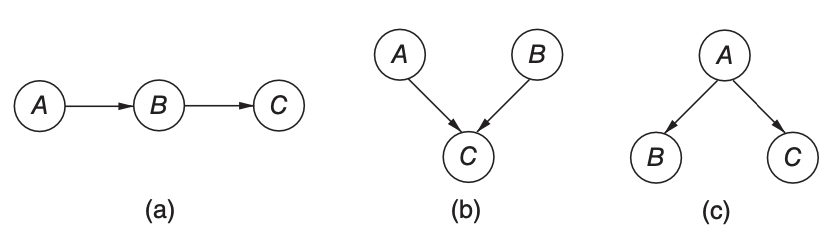
\includegraphics[scale=0.60]{slika4.png}
   \caption{Osnovne povezave v Bayesovih omrežjih:(a)zaporedna, (b)združevalna in (c)razhajajoča povezava.}\vspace{2mm}
\end{figure}
Zaporedna povezava je primerna, kadar presodimo, da poznavanje resničnega stanja $A$ zagotavlja relevantno informacijo o pojavu $B$ in poznavanje
resničnega stanja $B$ posledično zagotavlja relevantno informacijo o $C$, vendar ko je znano resnično stanje $B$, poznavanje stanja $A$ ne
zagotavlja več relevantne informacije o $C$. $A$ vpliva na $C$ preko $B$, vendar samo $B$ neposredno vpliva na $C$. Če je vrednost $B$ znana,
potem sta $A$ in $C$ verjetnostno neodvisna, tj. $P(C \lvert A, B) = P(C \lvert B)$.\\
\textit{Primer zaporedne povezave:\\} naj bodo hipoteze\\
$A \dots$ PoI je storilec kaznivega dejanja;\\
$B \dots$ Krvni madež, najden na kraju kaznivega dejanja, je od PoI;
$c \dots$ Vzorec krvi poškodovanca in krvni madež s kraja kaznivega dejanja imata enak profil DNK. \\
Potem je $A$ relevanten za $B$ in $B$ za $C$, vendar je lahko vzrok za prisotnost krvi glede na $B$ drugačen od $A$.\\\\
Pri združevalni povezavi za tri vozlišča $A$, $B$, $C$ sta $A$ in $B$ verjetnostno neodvisna, razen če je znana vrednost $C$ ali da sta $A$ in $B$
pogojno odvisna glede na vrednost $C$. Tako je $P(AB) = P(A) P(B)$, vendar $P(AB \lvert C) \ne P(A \lvert C) P(B \lvert C)$.\\
\textit{Primer združevalne povezave s tremi vozlišči $A$, $B$, $C$:\\} naj bo\\
$A \dots$ PoI je storilec kaznivega dejanja;\\
$B \dots$ Krvni madež, najden na kraju kaznivega dejanja, je od storilca kaznivega dejanja.\\
Če vemo, da se je eden od teh dogodkov zgodil, ne moremo pridobiti informacij o dogodku drugega, če pa je $C$ (krvni madež, najden na kraju
kaznivega dejanja, izvira od PoI) resničen, potem $A$ in $B$ postaneta povezana.\\\\
Pri razhajajoči se povezavi $A$ ločuje $B$ od $C$. Če je vrednost $A$ znana, potem sta $B$ in $C$ verjetnostno neodvisna, tj.
$P(B \lvert A, C) = P(B \lvert A)$ in $P(C \lvert A, B) = P(C \lvert A)$.

%%%%%%%%%%%%%%%%%%%%%%%%%%%%%%%%%%%%%%%%%%%%%%%%%%%%%%%%%%%%%%%%%%%%%%%%%%%%%%%%%%%%%%%%%%%%%%%%%%%%%%%%%%%%%%%%%%%%%%%%%%%%%%%%%%%%%%%%%%%%%%
\subsection{Uporaba Bayesovih omrežij na sodišču}
Bayesova omrežja, ki temeljijo na Bayesovi teoriji in teoriji grafov, ponujajo forenzičnim znanstvenikom več prefinjenih možnosti. Tem metodam
se daje poseben poudarek, kadar je treba med konkurenčnimi hipotezami izbrati najverjetnejšo, izbira pa mora biti podprta z znanstveno utemeljeno
argumentacijo. Primerna so za analizo dogodka, ki se je zgodil, in napovedovanje verjetnosti, da je k temu prispeval katerikoli od več možnih
znanih vzrokov. Prednosti Bayesovih mrež se najbolj izrazito pokažejo na zapletenih področjih z več spremenljivkami. Kriminalistične aplikacije
Bayesovih omrežij segajo od prepoznavanja storilcev, posameznih in kompleksnih konfiguracij različnih vrst sledi ter problemov sklepanja, ki
vključujejo rezultate analiz DNK.\\
Ti grafični modeli verjetnosti bistveno izboljšajo vrednotenje verjetnostnih razmerij, ki se uporabljajo za ocenjevanje znanstvenih dokazov.
Omogočajo, da se lotimo kompleksnejših verjetnostnih analiz, kot bi bilo to mogoče s tradicionalnimi pristopi. \\\\
Struktura BN v pravnem kontekstu je dovzetna za napačne predpostavke in napake v procesu ustvarjanja. Izbira vozlišč za dokaze je lahko
pristranska glede na to, kakšna vrsta argumenta je predstavljena. Argumenti obrambe ali tožilstva lahko na primer poudarjajo nasprotne sklepe
in zato vključujejo le podskupino dokazov. Če se za izdelavo ne uporablja dosleden okvir, lahko BN, ki jih oblikujejo različne stranke za en
primer, kažejo različne rezultate. Pri oblikovanju BN za pravno sklepanje je ključnega pomena, da se oblikuje omrežje, ki je razumljivo poroti
in sodniku.\\\\
Prikaz BN se mora ujemati z intuitivnim pripisovanjem vzročno-posledičnih povezav med končno hipotezo, kot je "Obtoženec je kriv.", podhipotezo
"Obtoženec je bil na kraju zločina." in dokazi primera. Poleg težav, ki se pojavijo med postopkom strukturiranja, je problematično tudi sklepanje
iz omrežja, če se izvaja ob napačnih predpostavkah. Verjetnosti, tudi če temeljijo na strokovni presoji, so lahko pristranske zaradi dejavnikov
motenj v postopku pridobivanja podatkov. Metode za sklepanje morajo zato zagotoviti, da se verjetnosti omrežij ne razlagajo napačno kot dejstva in
da se izpostavi dejavnik negotovosti. Primerjati morajo verjetnosti za nasprotujoče si hipoteze in morajo zagotoviti okvir za pravnike, da iz
mreže sklepajo na argumente.\\\\

%%%%%%%%%%%%%%%%%%%%%%%%%%%%%%%%%%%%%%%%%%%%%%%%%%%%%%%%%%%%%%%%%%%%%%%%%%%%%%%%%%%%%%%%%%%%%%%%%%%%%%%%%%%%%%%%%%%%%%%%%%%%%%%%%%%%%%%%%%%%%%
\subsection{Primer uporabe Bayesovega omrežja}

%%%%%%%%%%%%%%%%%%%%%%%%%%%%%%%%%%%%%%%%%%%%%%%%%%%%%%%%%%%%%%%%%%%%%%%%%%%%%%%%%%%%%%%%%%%%%%%%%%%%%%%%%%%%%%%%%%%%%%%%%%%%%%%%%%%%%%%%%%%%%%
%%%%%%%%%%%%%%%%%%%%%%%%%%%%%%%%%%%%%%%%%%%%%%%%%%%%%%%%%%%%%%%%%%%%%%%%%%%%%%%%%%%%%%%%%%%%%%%%%%%%%%%%%%%%%%%%%%%%%%%%%%%%%%%%%%%%%%%%%%%%%%
\section{Drugi pristopi}
Da bi ocenili moč Bayesove analize dokazov DNK, jo je koristno primerjati z nekaterimi drugimi pristopi.

%%%%%%%%%%%%%%%%%%%%%%%%%%%%%%%%%%%%%%%%%%%%%%%%%%%%%%%%%%%%%%%%%%%%%%%%%%%%%%%%%%%%%%%%%%%%%%%%%%%%%%%%%%%%%%%%%%%%%%%%%%%%%%%%%%%%%%%%%%%%
\subsection{Frekvence}
Predlagano je bilo s strani mnogih avtorjev, da je bolj naraven način za obravnavo verjetnosti uporaba naravnih frekvenc(angl. natural
frequencies).
\begin{definicija}
   Frekvenca $f$ je posamezno število diskretnih statističnih enot iste vrednosti. Če je diskretnih podatkov zelo veliko ali če so
   podatki zvezni, jih združujemo v frekvenčne razrede.
\end{definicija}

\begin{definicija}
   Absolutna frekvenca (oznaka $f_k$ za k-ti razred) je število vrednosti statistične spremenljivke v k-tem razredu.
\end{definicija}

\begin{definicija}
   Relativna frekvenca (oznaka $f_k'$) pa je delež absolutne frekvence $f_k$ glede na celoto. Če je $N$ število enot v populaciji
   ali morda vzorcu, je
   \[
       f_k' = \frac{f_k}{N}. \vspace{2mm}
   \]
\end{definicija}
V forenzičnem kontekstu se navedene frekvence običajno nanašajo na pojavljanje dokazov za posamezen primer, medtem ko se frekvence za
pojavljanje vprašanj običajno opisujejo kot osnovne stopnje(angl. base rates). Sklepanje o krivdi je lahko podprto s statistično analizo
ustreznih podatkov in verjetnostnim sklepanjem z uporabo absolutnih ali relativnih frekvenc, pri čemer je verjetnost, da bi določene
podatke (dokaze) pridobili zgolj po naključju, izjemno majhna . Relativne frekvence vedno navajajo ali predpostavljajo, da obstaja nek
referenčni vzorec, na podlagi katerega se lahko oceni pogostost zadevnega dogodka. Nadaljnja predpostavka je, da je ta primerjava poučna
in pomembna za obravnavano nalogo. V okviru kazenskega postopka bi na primer pričakovali, da bo relativna pogostost lahko podprla
vmesno sklepanje o moči dokazov, ki se nanašajo na sporna dejstva, kar vodi do končnega sklepa, da je obtoženec nedolžen ali kriv. Relativne
frekvence so rutinsko vključene v znanstvene dokaze, ki se predložijo v kazenskih postopkih.\\\\
Recimo, da je pogostost profila DNK $f$ 1 proti 10 milijonov, predpostavimo tudi, da ima obtoženec enak DNK in da je začetna populacija osumljencev
100 milijonov ljudi. Zanima nas kakšna je verjetnost, da je obtoženec vir DNK-ja s kraja zločina. \\
Naj bo: \\
$f$ \dots pogostost profila DNK;\\
$m$ \dots velikost populacije osumljencev; \\
$n$ \dots število ljudi, ki imajo ustrezen DNK profil. \\
Po metodah, ki temeljijo na naravnih frekvencah, je potrebno izračunati, koliko ljudi z zadevnim profilom DNK je v populaciji osumljencem, tako
da se $f$ pomnoži z $m$.  \\
Če je posameznikov s takim profilom $n > 1$, je verjetnost, da je obtoženi vir, $\frac{1}{n}$. V primeru, ko je $n < 1$ in so frekvence še
posebaj majhne, je bolje raziskovati ali je profil DNK edinstven ali ne - ali poleg obtoženca obstajajo še drugi posamezniki z enakim
profilom DNK. Temu pravimo metoda edinstvenosti(angl. uniqueness method). \\
S formulo binomske porazdelitve lahko izračunamo verjetnost, da se bo dogodek $X$, na primer profil DNK, pojavil $k$ - krat v $s$ - kratnem
številu ponovitev, pri čemer ima dogodek $X$ frekvenco 4$f$. Želimo vedeti, kolikšna je verjetnost, da ima točno en posameznik ustrezen DNK
profil, ob pogoju da ga ima vsaj en posameznik, torej:
\[
   P(n = 1 \lvert n \ge 1) = \frac{P(n=1 \cap n \ge 1)}{P(n \ge 1)} = \frac{m \times f \times (1 - f)^{m-1}}{1 - (1 - f)^m}. \vspace{2mm}
\]
\begin{table}[h!]
   \centering
   \begin{tabular}{c c c c}
       \hline
       $m$ & $f$ & $P(n = 1 \lvert n \ge 1)$ & $P(S \lvert M)$[Bayes]\\
       \hline
       10 milijonov & 1 v 100 milojonov & 0,9 & 0,9 \\
       100 milijonov & 1 v 100 milojonov & 0,62 & 0,5 \\
       1 milijarda & 1 v 100 milojonov & 0 & 0,09 \\ \hline
       10 milijonov & 1 v 1 milijardi & 1 & 0,99 \\
       100 milijonov & 1 v 1 milijardi & 0,9 & 0,9 \\
       1 milijarda & 1 v 1 milijardi & 0,62 & 0,5 \\ \hline
       10 milijonov & 1 v 10 milijardah & 1 & 0,999 \\
       100 milijonov & 1 v 10 milijardah & 1 & 0,99 \\
       1 milijarda & 1 v 10 milijardah & 0,9 & 0,9 \\ \hline
   \end{tabular}
\end{table}
Tabela vsebuje primerjavo rezultatov, ki jih daje Bayesovo pravilo. Obe metodi se dokaj ujemata, vendar se tudi razlikujeta, saj v nasprotju
z Bayesovim pravilom pri metodi edinstvenosti ni mogoče enostavno upoštevati številnih zapletov, kot je bil na primer vpliv stopnje
laboratorijskih napak.

%%%%%%%%%%%%%%%%%%%%%%%%%%%%%%%%%%%%%%%%%%%%%%%%%%%%%%%%%%%%%%%%%%%%%%%%%%%%%%%%%%%%%%%%%%%%%%%%%%%%%%%%%%%%%%%%%%%%%%%%%%%%%%%%%%%%%%%%%%%%
\subsection{Naključno ujemanje}
Metoda verjetnost naključnega ujemanja(angl. random match probability) izraža možnost, da bi imel naključni posameznik, ki ni povezan z obdolžencem,
ustrezni DNK profil. Ta verjetnost je enaka pogostosti profila DNK. Težava tega pristopa je, da verjetnost naključnega ujemanja lahko predstavljena
oziroma razumevana narobe. \\
Pogosto se to verjetnost interpretira na slednji način:
\begin{enumerate}
   \item če je verjetnost naključnega ujemanja na primer 1 proti 100 milijonom, potem je verjetnost, da ima profil DNK drug posameznik in ne
   obdolženec 1 proti 100 milijonom;
   \item ker je to zelo majhna verjetnost, mora biti tudi verjetnost, da je sled DNK pustil nekdo drug na kraju zločina in ne obdolženec, zelo majhna;
   \item zato mora biti verjetnost, da je vir sledi DNK s kraja zločina obtoženec zelo velika, ampak znaša 1 proti 100 milijonov.
\end{enumerate}
Takšno sklepanje je napačno in je znano kot tožilčeva zmota(angl. Prosecutor’s fallacy). Sestavlja jo enačba
\begin{equation}\label{eq:tozilcevazmota}
   1 - f = P(S \lvert M). \vspace{2mm}
\end{equation}
Zmota se pojavi v koraku (2), ko je zamenjano $P(M \lvert \neg S)$ s $P(\neg S \lvert M)$ in predpostavljeno, da sta obe verjetnosti enaki $f$. \\
Namesto verjetnosti naključnega ujemanja forenzični strokovnjaki pogosto pričajo o razmerju verjetnosti(angl. likelihood ratio) dokazov DNK, in
sicer kot:
\[
   P(M \lvert S) = P(M \lvert \neg S). \vspace{2mm}
\]
Bayesovo pravilo vključuje razmerje verjetnosti in predhodno oziroma pariorno verjetnost, torej je celovitejši način predstavitve dokazov DNK.
Težavo ocenjevanja apriorne verjetnosti pri Bayesovem pravilu, bi lahko odpravili z osredotočanjem le na verjetnost. Metoda razmerja verjetnosti je
koristna v državah kot sta na primer Velika Britanija in Združene države Amerike, kjer se lahko Bayesovo pravilo šteje kot poseg v pravico porote
do previdnosti: poroti naj ne bi bilo potrebno govoriti, kako naj razmišlja in presoja dokaze; Bayesovo pravilo pa je natanko metoda za
tehtanje dokazov.

%%%%%%%%%%%%%%%%%%%%%%%%%%%%%%%%%%%%%%%%%%%%%%%%%%%%%%%%%%%%%%%%%%%%%%%%%%%%%%%%%%%%%%%%%%%%%%%%%%%%%%%%%%%%%%%%%%%%%%%%%%%%%%%%%%%%%%%%%%%%
\subsection{Predhodna verjetnost(angl. Prior Probability)}
Sodni izvedenec je naprošen, da opravi analizo profila DNK krvi, najdene na kraju kaznivega dejanja, in rezultat primerja s profilom DNK
obdolženca. O krivdi ali nedolžnosti obtoženca bo odločala porota. Odločitev porotnikov bo delno odvisna od njihove ocene dveh interesnih
možnosti\\
$H_1 \dots$ vir krvi je obtoženec,\\
$H_2 \dots$ vir krvi je druga oseba.\\
Porotniki bodo morda želeli, da jim izvedenec dokončno pove, katera hipoteza je resnična, ali da jim navede posebne vrednosti tako imenovanih
verjetnosti vira. Za oceno verjetnosti vira mora forenzični znanstvenik upoštevati tudi druge dokaze v kazenskem primeru.\\\\
Recimo, da je izvedenec ugotovil, da imata obtoženec in kri s kraja zločina skupen niz genetskih označevalcev, ki jih najdemo pri eni osebi
na 1 milijon prebivalcev v zadevni populaciji. Ne da bi upošteval druge dokaze v zadevi, lahko izvedenec poda izjavo o pogojni verjetnosti
ugotovitve teh rezultatov pri dveh hipotezah o medsebojni povezanosti. Izvedenec lahko na primer izjavi, da so skupni genetski označevalci
skoraj zagotovo najdeni v primeru H1 (vir je bil obtoženec), vendar imajo le 1 možnost na milijon, da bodo najdeni v primeru $H_2$ (vir je bil
nekdo drug). Na podlagi te ocene lahko izvedenec poroti predloži razmerje verjetnosti - na primer, da so rezultati profiliranja DNK 1 milijonkrat
bolj verjetni, če je bil vir krvi obtoženec in ne neka druga oseba. Vendar razmerje verjetnosti ni isto kot verjetnost vira. \\
Edini skladen način, kako na podlagi forenzičnih dokazov sklepati o verjetnosti virov, je uporaba Bayesovega pravila, ki zahteva, da začnemo s
pripisom predhodnih verjetnosti za trditve, ki nas zanimajo. Bayesov pristop bo deloval le, če bo izvedenec lahko začel s predhodno verjetnostjo.\\\\
To nas pripelje do bistva vprašanja: ali naj forenziki sploh poskušajo določiti predhodne verjetnosti, in če da, kako. Občasno se predlaga, da
bi morali forenziki predpostavljati enake predhodne verjetnosti, kar se včasih opisuje kot stališče nevtralnosti. Torej analitiki predpostavljajo,
da sta predhodni verjetnosti $H_1$ in $H_2$ enaki, nato pa ju v skladu z Bayesovim pravilom pomnožijo z razmerjem verjetnosti, da določijo posteriorno
verjetnost. \\\\
Ampak kakršnakoli privzeta predpostavka o predhodni verjetnosti je obravnavana kot kršitev obveznosti pravnega sistema, da zagotovi individualizirano
pravico na podlagi dejstev vsakega primera, zato je drugi predlagani pristop, da forenzični znanstveniki prevzamejo odgovornost za oceno predhodne
verjetnosti ustreznih hipotez, preden jih posodobijo na podlagi znanstvenih ugotovitev v skladu z Bayesovim pravilom. Glavni očitek temu pristopu v
okviru kazenskega postopka je, da lahko forenzični znanstveniki presežejo svoje znanstveno znanje in si prisvojijo vlogo tistega, ki ugotavlja
dejstva. Da bi izvedenec določil predhodne kontekstualno smiselne verjetnosti, bi moral upoštevati vse dokaze v zadevi. Zato je bilo predlagano,
da sodni izvedenci nimajo nobene vloge pri ocenjevanju predhodnih verjetnosti. \\\\
Vprašanje, ali naj forenzični znanstveniki upoštevajo predhodno verjetnost hipotez, ki naj bi jih pomagali ovrednotiti, je zapleteno. Odgovor je odvisen od
vloge, ki jo bo forenzični znanstvenik imel v pravnem sistemu. Če bodo forenzični znanstveniki za pravne namene sprejemali ultimativne ugotovitve v zvezi z
določenim predlogom, ki jih zanima, potem bi morali in dejansko morajo upoštevati predhodne verjetnosti, da so hipoteze resnične. Če pa bo o
resničnosti hipotez odločal nekdo drug, npr. sodnik ali porota, in je vloga forenzičnih znanstvenikov omejena na zagotavljanje strokovne pomoči, se
morajo forenzični znanstveniki na splošno omejiti na določanje pogojne verjetnosti znanstvenih ugotovitev pri danih hipotezah, ki jih zanimajo, nalogo
ocenjevanja predhodnih in poznejših verjetnosti pa morajo prepustiti nosilcu pravne odločitve.

%%%%%%%%%%%%%%%%%%%%%%%%%%%%%%%%%%%%%%%%%%%%%%%%%%%%%%%%%%%%%%%%%%%%%%%%%%%%%%%%%%%%%%%%%%%%%%%%%%%%%%%%%%%%%%%%%%%%%%%%%%%%%%%%%%%%%%%%%%%%%%
%%%%%%%%%%%%%%%%%%%%%%%%%%%%%%%%%%%%%%%%%%%%%%%%%%%%%%%%%%%%%%%%%%%%%%%%%%%%%%%%%%%%%%%%%%%%%%%%%%%%%%%%%%%%%%%%%%%%%%%%%%%%%%%%%%%%%%%%%%%%%%
\section{Zmote v kazenskem pravu}
Ker večina ljudi pri razmišljanju o verjetnosti dela osnovne napake, obstaja mnogo zmot, ki izhajajo iz osnovnega razumevanja pravil
teorije verjetnosti. Številne od teh zmot so zlasti posledica napačnega razumevanja pogojne verjetnosti. Bolj znana primera takih zmot sta
Tožilčeva zmota(angl. Prosecutor’s fallacy) in Zmota obrambnega odvetnika(angl. Defense attorney's fallacy). Čeprav so posledice tožilčeve zmote
lahko hujše kot posledice zmote obrambnega odvetnika, so porote morda bolj dovzetne za slednjo kot za prvo. \\\\
Če upoštevamo vzročno verigo dokazov, predstavljeno na sliki 1, lahko razvrstitev zmot posplošimo na večino vrst dokazov. Ta shema
nam omogoča klasifikacijo napak v sklepanju.
\begin{figure}[!ht]\label{fig:slika_3}
   \centering
   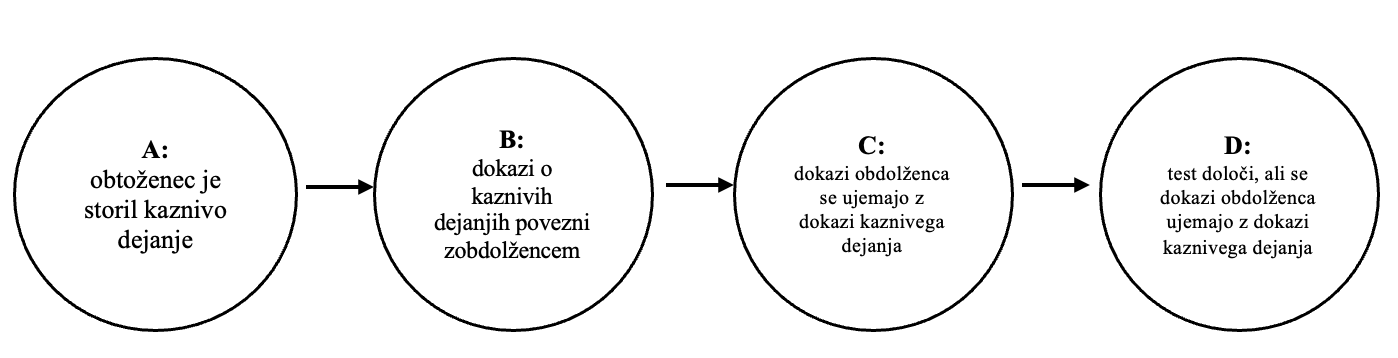
\includegraphics[scale=0.60]{slika_3.png}
   \caption{Vzorčna veriga dokazov}
\end{figure}
\\
Ta analiza je močno odvisna od pojma "pogostost ujemajočih se lastnosti", označenega kot $F$(lastnosti). Ta se včasih imenuje
tudi "verjetnost naključnega ujemanja". V našem vzročno-posledičnem okviru je $F$(lastnosti) enakovreden bolj formalno opredeljeni verjetnosti
$P(C \lvert \neg B)$, t.j. verjetnost, da oseba, ki ni vpletena v kaznivo dejanje, po naključju zagotovi dokaze, ki se ujemajo.\\\\
S tem vzročno-posledičnim okvirom lahko opišemo vrsto različnih pogostih zmot, ki so posledica napačnega razumevanja pogojne verjetnosti:\\
\textit{Napaka glavne težave}: pri tem enačimo $P(C \lvert \neg B)$ s $P(\neg A \lvert C)$. To je bilo
imenovano tožilska zmota - presega napako predhodne verjetnosti, saj si jo lahko predstavljamo kot dopolnitev te napake z dodatno napačno
predpostavko $P(A) = P(B)$.\\\\
\textit{Napaka verjetnosti $P(\text{drugo ujemanje})$}: gre za zmoto, ko verjetnost $P(C \lvert \neg B)$ enačimo z verjetnostjo
(imenujmo jo $q$), da ima vsaj en nedolžen član populacije ustrezne dokaze. Posledica te napake je običajno močno pretiravanje z vrednostjo
dokaza $C$.\\\\
\textit{Zanemarjanje predhodnih verjetnosti}: to pomeni preprosto neupoštevanje predhodnih vrednosti, kot sta $P(A)$ in $P(B)$. Na splošno
se za zmoto zanemarjanja osnovne stopnje šteje, kadar je verjetnost dogodka podcenjena, ker dogodek ni tako nenavaden, kot se zdi,
ali precenjena, ker je dogodek bolj nenavaden, kot se zdi.\\\\
\textit{Napaka pri številčnem preračunavanju}: pri tem gre za zamenjavo vrednosti $P(C \lvert \neg B)$ s pričakovanim številom drugih oseb,
ki bi jih bilo treba testirati, preden bi našli ujemanje. Ta zmota prav tako pretirava z vrednostjo dokaza $C$.\\\\
\textit{Pričakovane vrednosti, ki pomenijo edinstvenost}: če je velikost populacije približno enaka $1/P(\neg B \lvert C)$, potem mora biti
obdolženec edini primerek. Binomski izrek pokaže, da obstaja več kot 25\% verjetnost, da bosta v populaciji, katere velikost je $1/P(\neg B \lvert C)$,
vsaj dva ujemanja.\\\\
\textit{Zmota obrambnega odvetnika}: to se zgodi, ko se dokaz $C$ šteje za nepomembnega, ker visoka predhodna verjetnost $P(\neg A)$ (kar
se zgodi, če je na primer potencialno število osumljencev zelo veliko) še vedno povzroči visoko verjetnost $P(\neg B \lvert C)$.
\textit{Napaka baze podatkov obrambnega odvetnika}: za to napako gre, kadar verjetnost $P(\neg B \lvert C)$ temelji na drugačni populaciji,
kot jo določa $P(B)$ ali $P(A)$.\\\\
\textit{Zasliševalčeva zmota}: v tem primeru je dokaz neposredno priznanje krivde. Če to ni potrjeno, to pomeni, da uporabljamo $P(D \lvert A)$ za
informiranje $P(A \lvert D)$. Napaka je, da ne upoštevamo $P(D \lvert \neg A)$. Če je $P(D \lvert A) \leq P(D \lvert \neg A)$, potem dokaz
nima vrednosti.\\\\
Poleg zmot, ki izhajajo iz osnovnega nerazumevanja pogojne verjetnosti, se druge zmote pojavijo zaradi neustreznega združevanja vpliva več dokazov:\\
\textit{Zmota odvisnih dokazov}: ta zmota, ki se včasih imenuje tudi dvojno štetje, se kaže v tem, da se dva ali več dokazov, ki so odvisni,
obravnava, kot da bi bili neodvisni, zaradi česar je izjava o njihovi skupni verjetnosti manjša, kot bi morala biti. Poseben primer te zmote je
\textit{logično odvisna dokazna zmota}, pri kateri en dokaz ni preprosto odvisen od drugega, ampak dejansko logično izhaja iz njega.\\\\
\textit{Napaka konjunkcije}: ta zmota se pojavi, kadar preiskovalec ne upošteva dejstva, da je dokaz sestavljen iz več kot enega negotovega dogodka,
in mu posledično pripiše večjo verjetnost, kot bi jo moral.\\\\

%%%%%%%%%%%%%%%%%%%%%%%%%%%%%%%%%%%%%%%%%%%%%%%%%%%%%%%%%%%%%%%%%%%%%%%%%%%%%%%%%%%%%%%%%%%%%%%%%%%%%%%%%%%%%%%%%%%%%%%%%%%%%%%%%%%%%%%%%%%%%%
%%%%%%%%%%%%%%%%%%%%%%%%%%%%%%%%%%%%%%%%%%%%%%%%%%%%%%%%%%%%%%%%%%%%%%%%%%%%%%%%%%%%%%%%%%%%%%%%%%%%%%%%%%%%%%%%%%%%%%%%%%%%%%%%%%%%%%%%%%%%%%
\section{Tožilčeva zmota}
Verjetnostno utemeljevanje pravnih dokazov se torej skrči na preprost vzročni scenarij: začnemo z neko hipotezo $H$ in opazujemo nek dokaz $E$.
Poznavanje pogojne verjetnosti $P(E \lvert H)$ nam omogoča, da spremenimo svoje prepričanje o verjetnosti $H$, če poznamo $E$. Veliko najpogostejših
napak v sklepanju izhaja iz osnovnega nerazumevanja pogojne verjetnosti. Še posebej pogost primer je zamenjava verjetnost dokaza $E$ glede na
hipotezo $H$ z verjetnost hipoteze $H$ glede na dokaze $E$ oziroma $P(E \lvert H)$ z $P(H \lvert E)$. To se pogosto imenuje napaka prenesenega pogojnika
oziroma tudi tožilčeva zmota.\\\\
Tožilčeva zmota(angl. Prosecutor’s fallacy) se pogosto pojavlja v kazenskem pravu, vendar jo pogosto neprepoznajo, deloma zato, ker preiskovalci
nimajo močne intuicije o tem, kaj zmota sploh pomeni. Tožilčeva zmota je dobro znana statistična zmota, ki izhaja iz napačnega razumevanja
pogojnih verjetnosti in vprašanj večkratnega testiranja. Napaka temelji na predpostavki, da je $P(H \lvert E) = P(E \lvert H)$, pri čemer $H$
predstavlja primer, da se najdejo dokazi o obtožencu, $E$ pa primer, da je obtoženec nedolžen. Vendar ta enakost ne drži: čeprav je $P(H \lvert E)$
običajno zelo majhen, je lahko $P(E \lvert H)$ še vedno veliko večji. \\\\
Za lažjo predstavo si oglejmo primer. Na primer, da ima storilec zločina enako krvno skupino kot obtoženec in da ima 10\% prebivalstva
enako krvno skupino. Potem je lahko na podlagi tega verjetnost, da je obtoženec kriv, 90 odstotna. Vendar je ta sklep skoraj pravilen le, če
je bil obtoženec izbran kot glavni osumljenec na podlagi trdnih dokazov, ki so bili odkriti pred krvnim testom in z njim nispo povezani, saj
je lahko ujemanje krvi popolno naključje. V nasprotnem primeru je predstavljena utemeljitev napačna, saj ne upošteva predhodne verjetnosti, da
gre za naključno nedolžno osebo. Denimo, da v mestu, kjer se je zgodil zločin, živi 1000 ljudi. To pomeni, da tam živi 100 ljudi, ki imajo
krvno skupino storilca, zato je verjetnost, da je obtoženec kriv - na podlagi dejstva, da se njegova krvna skupina ujema s krvno skupino
morilca - le 1\%, kar je veliko manj kot 90\%. \\\\
Do tožilčeve zmote lahko pride zaradi večkratnega testiranja, na primer pri primerjanju dokazov z veliko podatkovno bazo. Velikost podatkovne
zbirke povečuje verjetnost, da bo ujemanje ugotovljeno zgolj po naključju. \\\\
Če je $E$ dokaz in $H$ trditev,da je obtoženi nedolžen, upoštevamo pogojne verjetnosti: \\
$P(E \lvert H)$ \dots verjetnost resničnosti dokaz $E$, kljub temu da je obtoženi nedolžen; \\
$P(H \lvert E)$ \dots verjetnodt, da je obtoženi nedolžen kljub dokazu $E$. \\
Pri forenzičnih dokazih je ponavadi verjetnost $P(E \lvert H)$ majhna. Tožilec pa potem velikokrat sklepa, da je tudi verjetnost
$P(H \lvert E)$ majhna.
%(tožilstvo Lucie de Berk je na primer obtoženo ravno te napake)
Zgoraj napisani pogojni verjetnosti pa sta precej različni; uporabimo Bayesovo pravilo:
\[
   P(H \lvert E) = P(E \lvert H) \times \frac{P(H)}{P(E)}, \vspace{2mm}
\]
kjer je $P(H)$ verjetnost nedolžnosti in $P(E)$ verjetnost dokaza. Enačba kaže, da majhna pogojna verjetnost $P(E \lvert H)$ ne pomeni majhne
pogojne verjetnosti $P(H \lvert E)$ v primeru velike verjetnosti nedolžnosti in majhne verjetnosti dokaza. \\
Po Bayesovem pravilu je
\[
   P(E)=P(E \lvert H)P(H) + P(E \lvert \neg H)\times[1 - P(H)] \vspace{2mm}
\]
kjer je $P(E \lvert \neg H)$ verjetnost, da bodo dokazi identificirali krivega osumljenca; bičajno je ta verjetnost blizu 1.

%%%%%%%%%%%%%%%%%%%%%%%%%%%%%%%%%%%%%%%%%%%%%%%%%%%%%%%%%%%%%%%%%%%%%%%%%%%%%%%%%%%%%%%%%%%%%%%%%%%%%%%%%%%%%%%%%%%%%%%%%%%%%%%%%%%%%%%%%%%%
\subsection{Primer - Tožilčeva zmota}
Slika 1 prikazuje populacijo 100 moških, starih 50 let, ki se ne zdravijo zaradi hipertenzije in imajo skupni holesterol 235 mg/dl in krvni tlak 120 mmHg. Pričakuje
se, da bo 9\% teh moških (predstavljeno z devetimi črtastimi kvadrati) čez 10 let imelo miokardni infarkt(MI). Ena četrtina moških je kadilcev (predstavljeno s 25
sivimi kvadrati); približno 16\% naj bi bilemo MI v 10 letih; zato bo $\frac{4}{25}$ kadilcev imelo MI (predstavljeno s črtastimi in sivimi kvadrati). \\
Število kadilcev, ki imajo MI, je očitno enako številu ljudi, ki imajo MI in so kadilci. Toda ali je delež kadilcev, ki imajo MI, enak deležu ljudi z MI, ki so kadilci? Iz
slike 1 je odogovor očitno ne; verjetnost, da ste kadilec glede na to, da ste imeli MI, torej:
\[
   P(\text{MI} \lvert \text{kadilec}) \ne P(\text{kadilec} \lvert \text{MI}), \vspace{2mm}
\]
ker
\[
   P(\text{MI} \lvert \text{kadilec}) = P(\text{črtasto} \lvert \text{sivo}) = \frac{4}{25} = 0,16 \vspace{2mm}
\]
in
\[
   P(\text{kadilec} \lvert \text{MI}) = P(\text{sivo} \lvert \text{črtasto}) = \frac{4}{9} = 0,44. \vspace{2mm}
\]
Vizualno opazimo, da delež sivih kvadratov, ki se prekrivajo s črtastimi kvadrati, ni enak deležu črtastih kvadratov, ki se prekrivajo s sivimi kvadrati.
\begin{figure}[!ht]\label{fig:slika1}
   \centering
   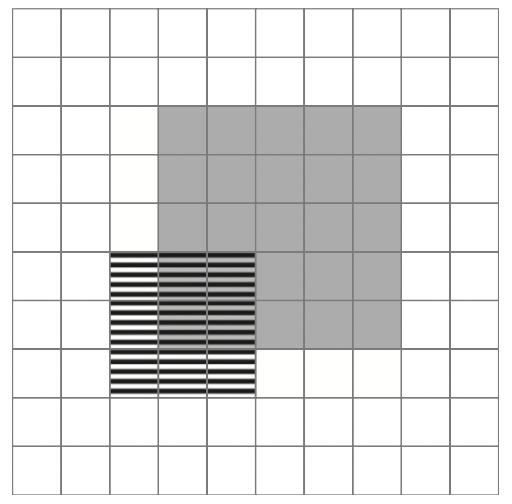
\includegraphics[scale=0.45]{slika1.png}
   \caption{Populacija, predstavljena s 100 kvadrati, z 9 črtastimi, 25 sivimi in 4 črtastimi in sivimi}\vspace{2mm}
\end{figure}
Slika 2 prikazuje izjeme pri tožilčevi zmoti, predstavljeni na sliki 1. Sedaj imamo 16 črtastih kvadratov, 16 sivih in 4 pikčaste in sive kvadrate, ker je splošna
razširjenost črtastih in sivih kvadratov enaka, je
\[
   P(\text{črtasto} \lvert \text{sivo}) = P(\text{sivo} \lvert \text{črtasto}). \vspace{2mm}
\]
Tudi
\[
   P(\text{črtasto} \lvert \text{pikčasto}) = P(\text{pikčasto} \lvert \text{črtasto}), \vspace{2mm}
\]
saj sta obe verjetnosti enaki $0$. Oboje(podobno velike populacija in populacije brez prekrivanja) je ozka izjema zmote. \\
Po drugi strani pa so črtkani kvadrati na sliki 2 v celoti zajeti v sivih kvadratih; tako je
\[
   P(\text{sivo} \lvert \text{črtkano}) = 1, \quad \text{medtem ko je} \quad P(\text{črtkano} \lvert \text{sivo}) = 0,25. \vspace{2mm}
\]
Tožilčeva zmota velja, kadar je ena skupina podmnožica druge.

\begin{figure}[!ht]\label{fig:slika2}
   \centering
   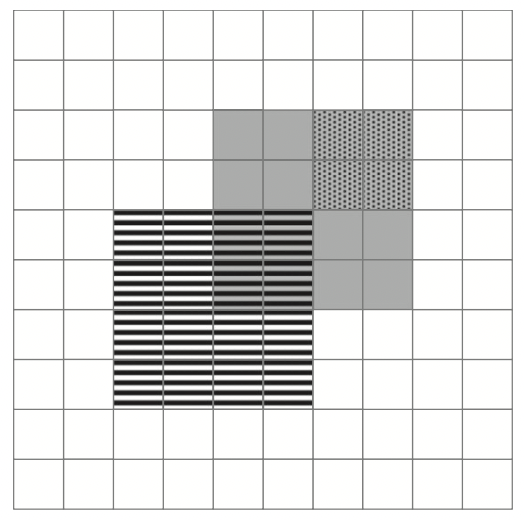
\includegraphics[scale=0.45]{slika2.png}
   \caption{Populacija, predstavljena s 100 kvadrati, z 16 črtastimi, 16 sivimi in 4 pikčastimi in sivimi}\vspace{2mm}
\end{figure}

%%%%%%%%%%%%%%%%%%%%%%%%%%%%%%%%%%%%%%%%%%%%%%%%%%%%%%%%%%%%%%%%%%%%%%%%%%%%%%%%%%%%%%%%%%%%%%%%%%%%%%%%%%%%%%%%%%%%%%%%%%%%%%%%%%%%%%%%%%%%%%
%%%%%%%%%%%%%%%%%%%%%%%%%%%%%%%%%%%%%%%%%%%%%%%%%%%%%%%%%%%%%%%%%%%%%%%%%%%%%%%%%%%%%%%%%%%%%%%%%%%%%%%%%%%%%%%%%%%%%%%%%%%%%%%%%%%%%%%%%%%%%%
\section{Izogibanje zmotam z uporabo razmerja verjetnosti}
Vsem zgoraj opisanim zmotam je skupno to, da je resnična koristnost dokaza predstavljena na zavajajoč način - bodisi je pretirana bodisi podcenjena.
Prednost uporabe razmerja verjetnosti je, da odpravlja ugovorov Bayesovemu izreku, in sicer obveznost upoštevanja predhodne verjetnosti za hipotezo,
kot je "kriv" (tj. kot sta A ali B na sliki 3, nam ni treba upoštevati predhodne verjetnosti). V veliki meri pomiri pomisleke pravnikov,
ki bi sicer zavrnili Bayesov argument z utemeljitvijo, da je nedopustno predpostavljati predhodne verjetnosti o krivdi ali nedolžnosti.\\\\
Čeprav je uporaba razmerja verjetnosti kot sredstva za izogibanje zmotam in merjenje uporabnosti dokazov močno podprta, sem vseeno mnenja, da
imajo, po prebiranju različnih sodb, pravniki in laiki pogosto podobne težave pri razumevanju razmerja verjetnosti kot pri razumevanju
Bayesove teorije.

%%%%%%%%%%%%%%%%%%%%%%%%%%%%%%%%%%%%%%%%%%%%%%%%%%%%%%%%%%%%%%%%%%%%%%%%%%%%%%%%%%%%%%%%%%%%%%%%%%%%%%%%%%%%%%%%%%%%%%%%%%%%%%%%%%%%%%%%%%%%%%
%%%%%%%%%%%%%%%%%%%%%%%%%%%%%%%%%%%%%%%%%%%%%%%%%%%%%%%%%%%%%%%%%%%%%%%%%%%%%%%%%%%%%%%%%%%%%%%%%%%%%%%%%%%%%%%%%%%%%%%%%%%%%%%%%%%%%%%%%%%%%%

%%%%%%%%%%%%%%%%%%%%%%%%%%%%%%%%%%%%%%%%%%%%%%%%%%%%%%%%%%%%%%%%%%%%%%%%%%%%%%%%%%%%%%%%%%%%%%%%%%%%%%%%%%%%%%%%%%%%%%%%%%%%%%%%%%%%%%%%%%%
%%%%%%%%%%%%%%%%%%%%%%%%%%%%%%%%%%%%%%%%%%%%%%%%%%%%%%%%%%%%%%%%%%%%%%%%%%%%%%%%%%%%%%%%%%%%%%%%%%%%%%%%%%%%%%%%%%%%%%%%%%%%%%%%%%%%%%%%%%%%
% Seznam uporabljene literature
%https://www.quantstart.com/articles/Bayesian-Statistics-A-Beginners-Guide/
%https://en.wikipedia.org/wiki/Prosecutor%27s_fallacy
%https://www.researchgate.net/publication/267131008_The_interrogator%27s_fallacy
%https://en.wikipedia.org/wiki/Bayesian_network


\end{document}